(\chapter{Background}\label{chap:background}
To predict the next element in a running case, we bring together the domains of Process Science, Predictive Modeling and Deep Learning. This background chapter gives comprehensive insight into those parts of said domains which will be used and referenced in this thesis. The chapter approaches them in a top-down fashion, starting with the high-level perspective from Process Science and how Process Mining is distinguished from Predictive Process Monitoring in \autoref{sec:process-science}. The section ends with information on how the used logs usually come into existence and which requirements these logs need to fulfill to be used in a prediction scenario.
With the data origin explained, \autoref{sec:predictive-modeling} introduces a process along which predictive model development usually takes place.
\autoref{sec:artificial-neural-networks} gives an in-depth look at neural networks and the components relevant to this thesis, especially stressing the importance of long short-term memory cells.
Finally, \autoref{sec:background:feature-engineering} highlights the peculiarities encountered when dealing with sequential data and introduces popular approaches to deal with them.

\section{Process Science}\label{sec:process-science}
Business processes are a collection of structured tasks which serve a particular business goal, if ordered in a specific sequence~\cite{weske2012business}. To facilitate a common understanding of a process, processes are visualized with modeling languages~\cite{panagacos2012ultimate}. Most languages, for example the Business Process Modeling Notation (BPMN)~\cite{bpmn2.0}, model the process flow in steps, commonly referred to as \textit{activities} - shown in \autoref{fig:activity-introduction}. An instance of a process is referred to as case.

\begin{figure}[!htb]
    \centering
    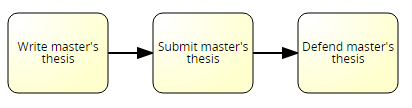
\includegraphics[width=.75\textwidth]{gfx/activity-introduction.png}
    \caption[Control flow in BPMN]{The yellow boxes and their description are used in BPMN to describe an activity, while the arrows denote the control flow in between}
    \label{fig:activity-introduction}
\end{figure}

Process Science, as loosely defined by van der Aalst~\cite{Aalst2016}, refers to the "broader discipline that combines knowledge from information technology and knowledge from management sciences to improve and run operational processes".

With the help of workflow management systems (WFMS), it is possible to embed and enforce business processes in an organization. When an activity in a process is executed, it goes through different stages. These stages are captured in the activity lifecycle in \autoref{fig:activity-lifecycle}. WFMS log events related to each activity, but the types of captured events are specific to the modeling language and the execution environment of the WFMS.

\begin{figure}[!htb]
    \centering
    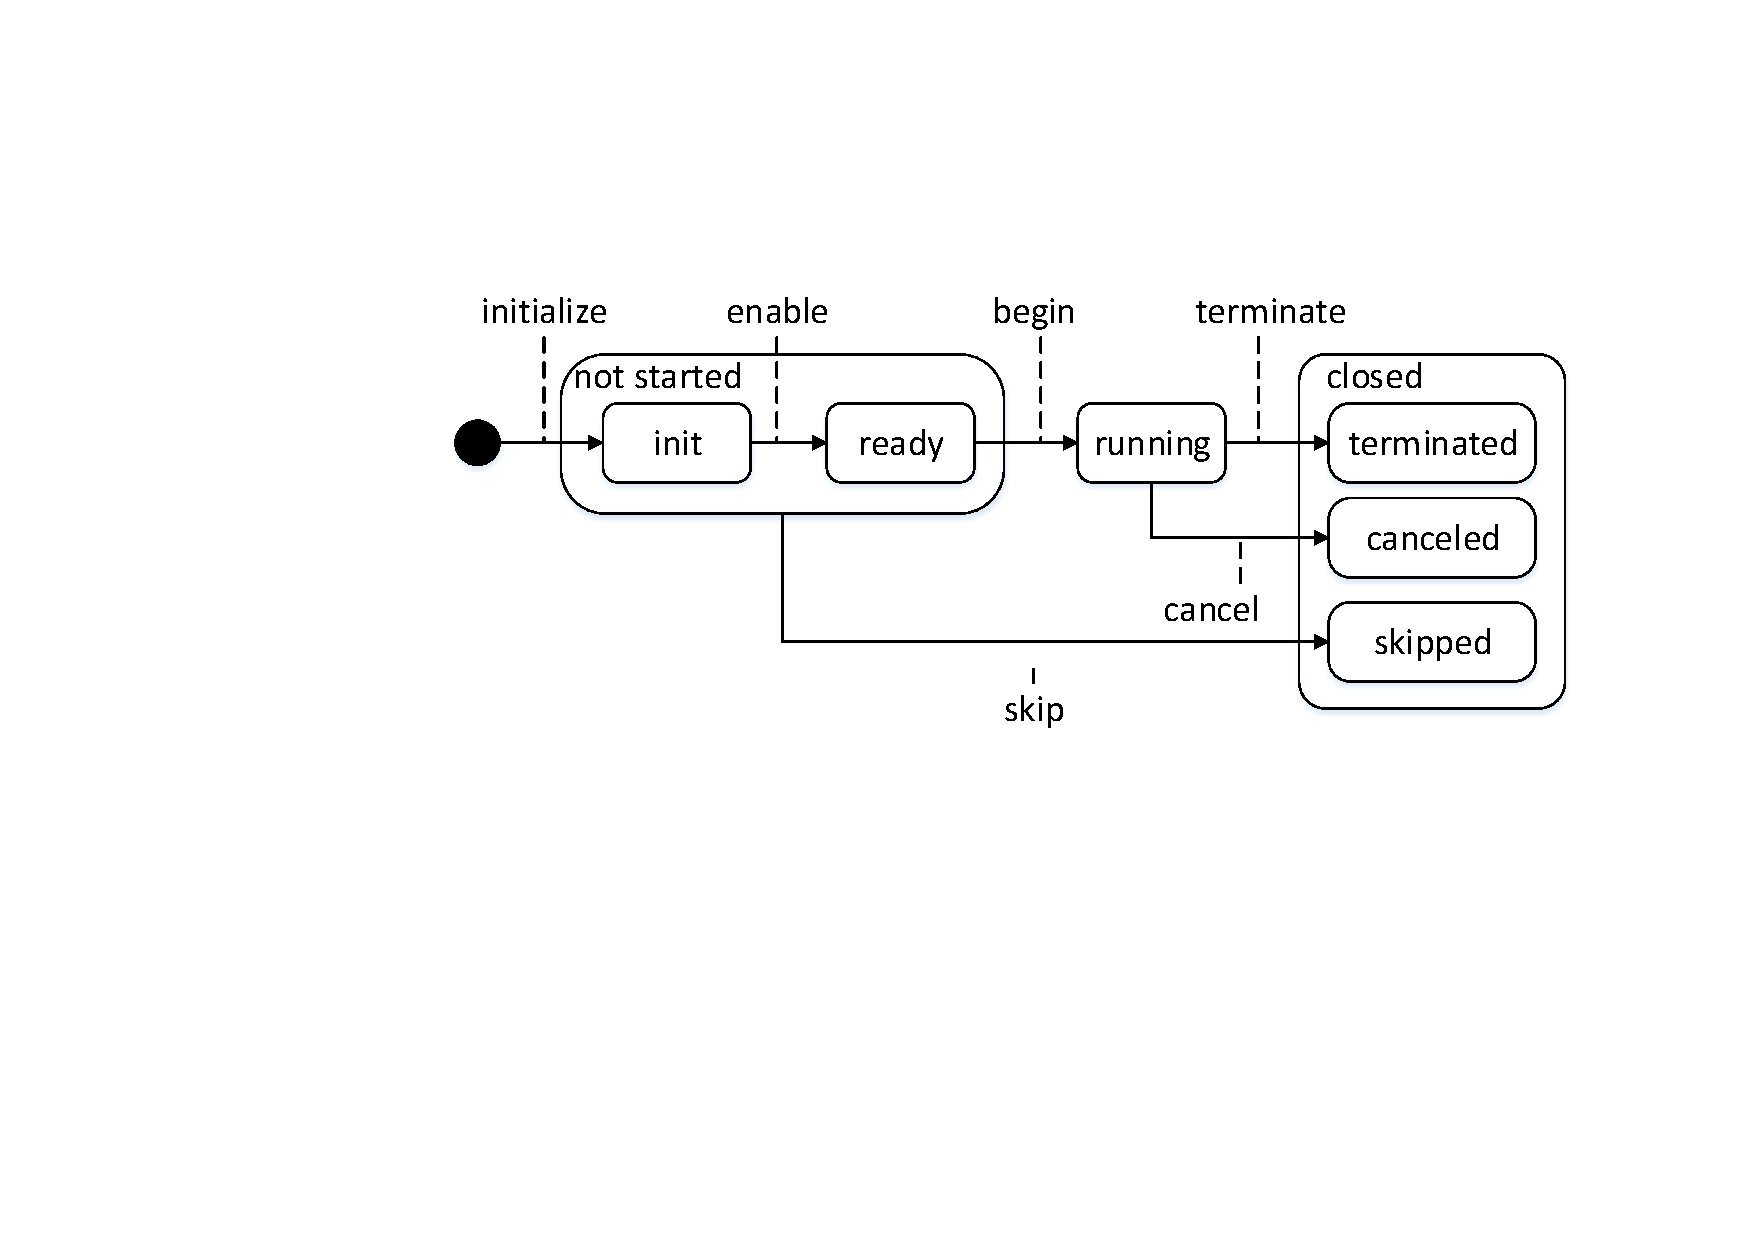
\includegraphics[width=.9\textwidth]{gfx/activityLifeCycle.pdf}
    \caption{The activity lifecycle}
    \label{fig:activity-lifecycle}
\end{figure}

The event logs give rise to the disciplines of Process Mining and Predictive Process Monitoring, as their analyses are based on the information contained in those logs~\cite{Aalst2016}. Because of the paramount importance of logs for this work, this section begins with \autoref{sec:log-structure} defining the properties and structure of a log. \autoref{sec:process-mining} and \autoref{sec:predictive-process-monitoring} contrast Process Mining and Predictive Process Monitoring.

\subsection{Process logs}\label{sec:log-structure}
A process log tracks the execution history of a process and can be understood in a hierarchical manner. Each log of a process consists of cases, which represent instances of a process. A case itself consists of a trace of events, i.e. a sequence that only belongs to a single case. Each event can have attributes attached~\cite{Aalst2016}.

\begin{figure}
    \centering
    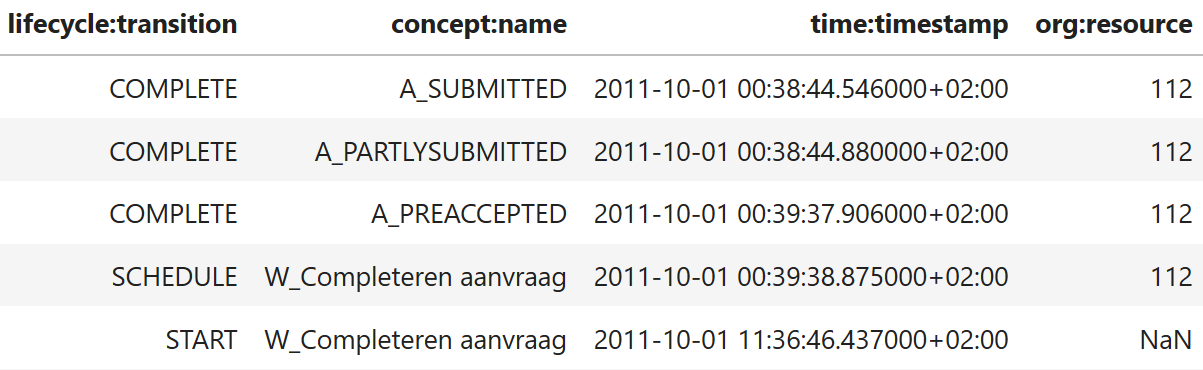
\includegraphics[width=\textwidth]{gfx/process-log.png}
    \caption{A case excerpt from BPIC11}
    \label{fig:process-log}
\end{figure}

Process event logs are typically made availble via XES files. XES is an abbreviation for the \textit{eXtensible Event Stream} standard~\cite{gunther2013xes}. An excerpt from a case extracted from the BPIC11 XES file~\cite{BPIC2011} is displayed in \autoref{fig:process-log}. In this particular log, only completion events are tracked, as evidenced by the values in the \verb=lifecycle:transition= column.\\

Formally, a log is defined as follows~\cite{Aalst2016}. It is made up of cases $c \in \mathscr{C}$, where $\mathscr{C}$ is the case universe. Similar to events, cases have attributes, e.g. a name. The operator $\#_{attr}(c)$ returns the value of the attribute $attr$ on a case $c$. A mandatory attribute of any case is its trace $\#_{trace}(c)$, which is especially relevant for our work.
Each trace represents a finite sequence of events $e \in \mathscr{E}$:

$$ \#_{trace}(c) = \langle e_1, e_2, e_3 \dots, e_n \rangle $$

The events are ordered by timestamp. In turn, each event $e$ has certain attributes associated with it. It is assumed that for a specific process, the type, number and name of these attributes does not change. An example for common attributes are the activity name $\#_{activity}(e)$ or the timestamp $\#_{timestamp}(e)$ at which the event occurred. Coming back to the example in \autoref{fig:process-log}, $e = \#_{trace}(c)[2]$ would get the second event in the trace, and $\#_{lifecycle:transition}(e)$ would produce the value \verb=complete=.
\todo[inline]{Übergang?}

\subsection{Process Mining}\label{sec:process-mining}
Process Mining covers the three steps of process model discovery, conformance checking and process model enhancement \cite{Aalst2016} -  all based on process event logs. It is worth noting that the logs can be enriched with data from systems other than WFMS. The three steps are enabled with techniques from Data Science, making it possible to understand Process Mining as a link between Data Science and Process Science. This is also visualized in \autoref{fig:process-data-science}.

\begin{figure}[!htb]
    \centering
    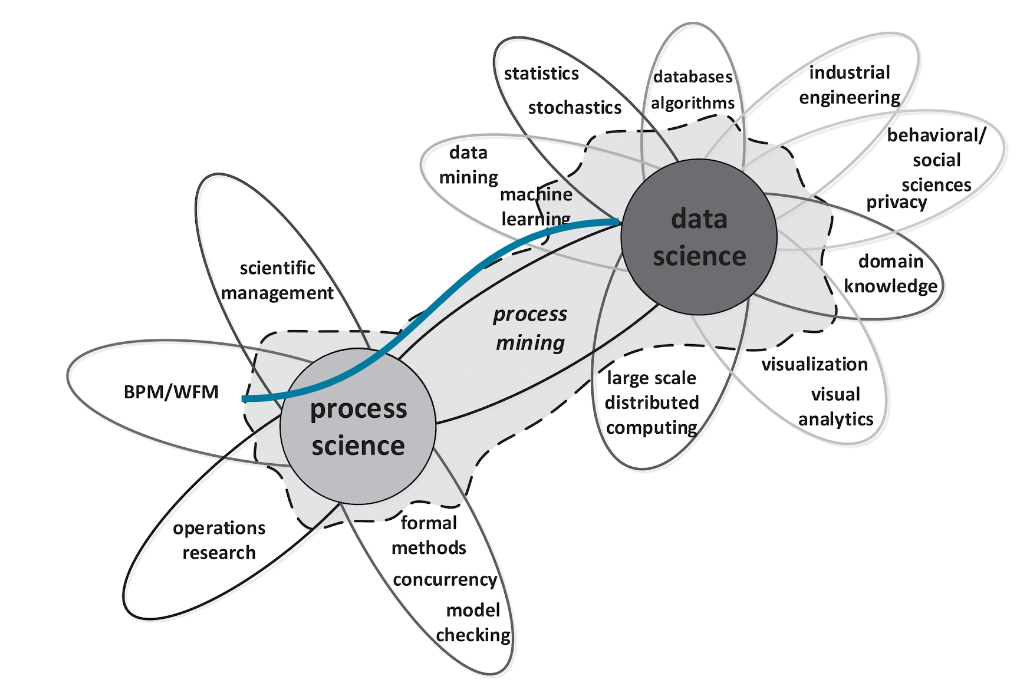
\includegraphics[width=.8\textwidth]{gfx/process-data-science.png}
    \caption[Process Mining connects two disciplines]{Process Mining connects Process Science and Data Science \cite[p.18]{Aalst2016} - the blue line symbolizes the subdomains that Predictive Process Monitoring brings together}
    \label{fig:process-data-science}
\end{figure}

A major problem when discovering process models is posed by spaghetti and lasagna process models~\cite{Aalst2016}. These overly complex and unreadable models are mined from process logs that contain highly variable execution traces. Because Process Mining revolves around process models, and the data-driven discovery and optimization based on historical data, a possibility to act on case developments in real-time without model-imposed restrictions is desirable. Predictive Process Monitoring provides this possibility.

\FloatBarrier
\subsection{Predictive Process Monitoring}\label{sec:predictive-process-monitoring}
Predictive Process Monitoring is aimed at the use of online data to make statements about the progression of a running case~\cite{francescomarino2015, schoenig2018}. It is not based on process models, but predictive models, and thus provides a flexibility that is not available within model-based Process Mining.  As visualized in \autoref{fig:process-data-science}, Predictive Process Monitoring connects two sub-domains of Process Science and Data Science. This makes it a discipline within Process Mining~\cite{Aalst2016}. With Predictive Process Monitoring, questions such as the following can be answered:

\begin{enumerate}
    \item Can the service level agreement still be met?
    \item How long is this case still going to take?
    \item What is going to be the next step in the case?
\end{enumerate}

The answers to these questions can give case workers the opportunity to intervene if a case takes an unwanted course or might fail to meet requirements. Furthermore, this approach only requires sufficient amounts of historical case executions to train the predictive models. What this entails is explained in the following chapter.

\section{Predictive Modeling}\label{sec:predictive-modeling}
Predictive Modeling is a domain that deals with creating models from learned statistical properties of data to predict outcomes~\cite{sivaganesan1994predictive}. These models are referred to as predictive models, and are not related to process models. This section introduces a common process for predictive model generation in \autoref{sec:predictive-model-development}.
As we aim to transfer a method from NLP to Predictive Process Monitoring, we introduce a definition of sequences in \autoref{sec:background:sequences}. Then, we frame the problem in \autoref{sec:background:sequence-prediction} that is fundamental to this thesis: next-element predictions in a sequence.

\subsection{Predictive model development}
\label{sec:predictive-model-development}
\begin{figure}
	\centering
	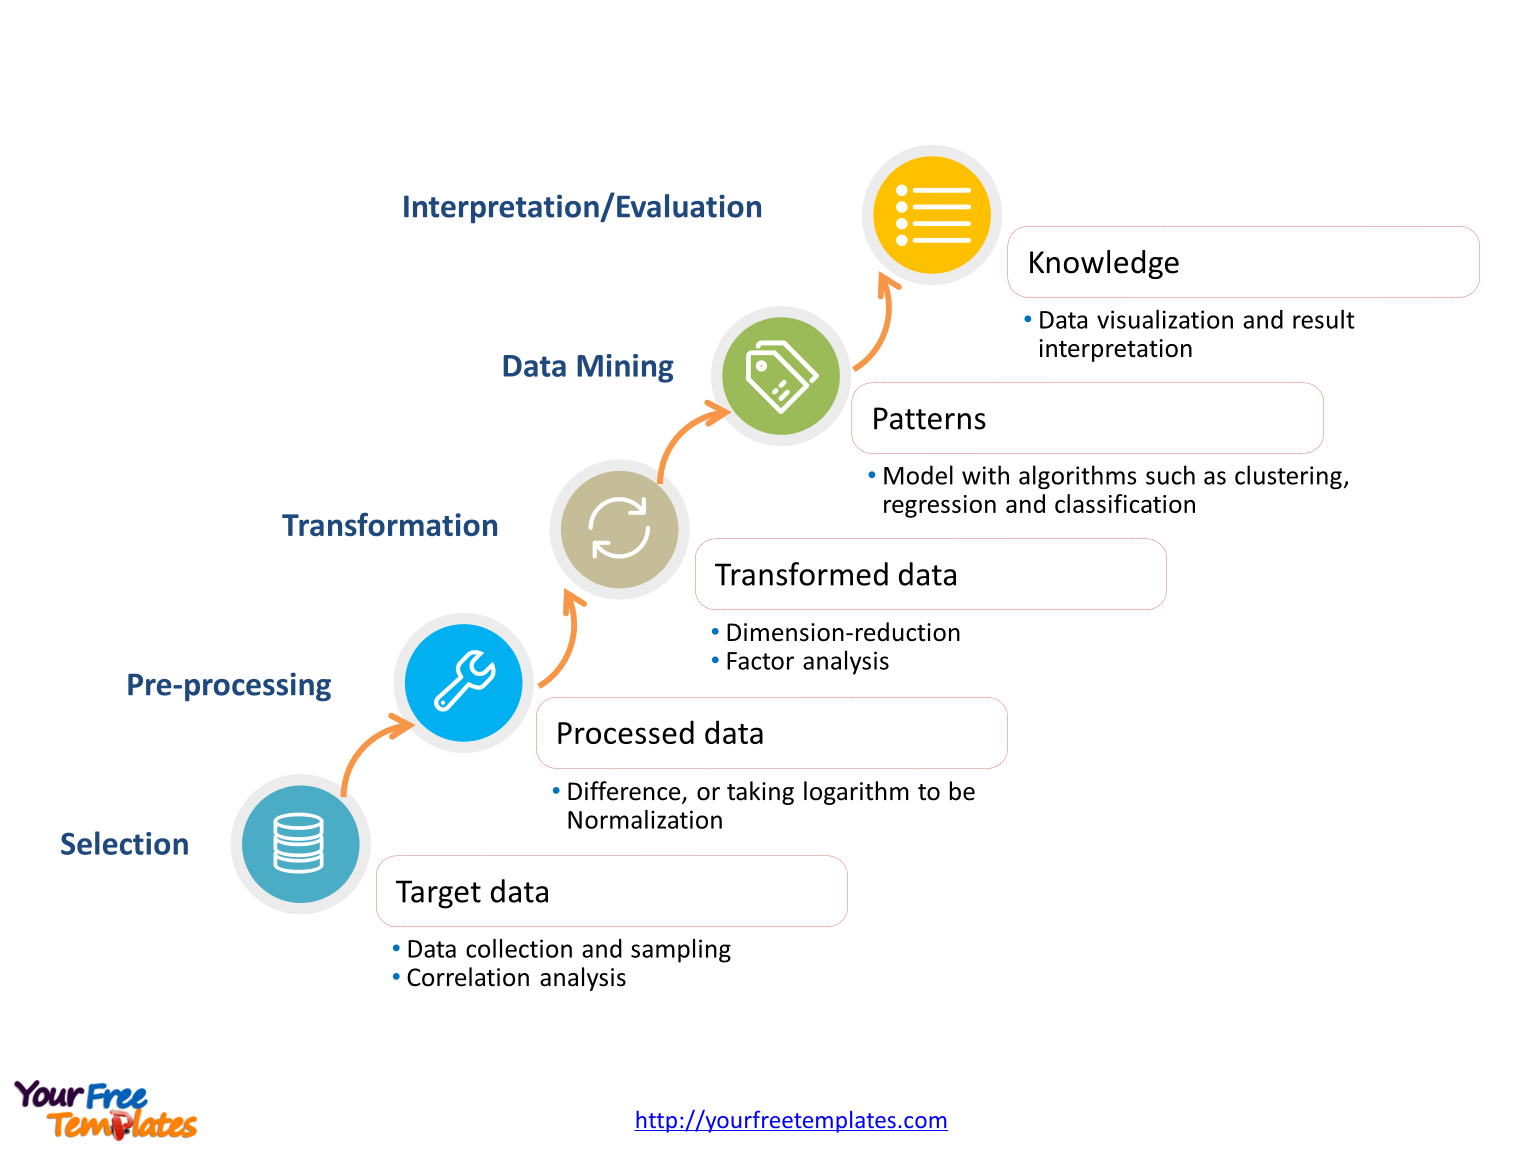
\includegraphics[width=\textwidth]{gfx/kdd_process.png}
	\caption{The process for \textit{Knowledge Discovery in Databases}~\cite{fayyad1996data}}
	\label{fig:kdd_process}
\end{figure}
In 1996 Fayyad et al. published what came to be known as the Knowledge Discovery in Databases (KDD) process~\cite{fayyad1996data}. Published over 20 years ago and aimed at data mining, it is also applicable to predictive model building. It is illustrated in \autoref{fig:kdd_process}, and shall be explained step by step in the following with technical details relevant for this thesis. The process is highly iterative, is focused intensely on the data, and jumps between every step are possible~\cite{kuhn2013applied}.\\

Predictive models are the statistical tools that are used to make predictions. They work on \textit{samples}, which are comprised of a number of \textit{features} - variables that are considered useful for the prediction of the \textit{target variable}. The target variable may either be a continuous or discrete value. In the latter case, the output is referred to as classification. Activities are discrete, and as such this thesis deals with classification. In the exemplary log in \autoref{fig:process-log}, each row can be understood as a sample and each column as a single feature. Features are sometimes also referred to as predictor variables.

\subsubsection*{Selection}
During the first step of the KDD process in \autoref{fig:kdd_process}, features are chosen as predictors based on differed criteria such as their predictive power or inter-feature correlations. Based on the latter, features can also be omitted from the original dataset.

\subsubsection*{Pre-processing}
The second step of the KDD process is focused on data quality. Features may be sparse or contain data of low quality, i.e. different spelling of the same entity or typing errors. With data cleansing, these issues are resolved and appropriate values imputed where they are missing.

\subsubsection*{Transformation}\label{sec:predictive-model-development:transformation}
The third step of the KDD process is aimed at making the data accessible for machine learning methods. During transformation, some features might be aggregated, normalized or encoded differently to assist the predictive model in picking up relations between variables. Common tasks are one-hot or dictionary encoding of discrete values such as strings, e.g. activity names. Variable concatenations or complex aggregations might also be added as \textit{engineered} features~\cite{kuhn2013applied}.

\subsubsection*{Data Mining}
Data mining deals with the extraction of implicit, previously unknown, and potentially useful information from data. Machine learning provides a technical basis for this~\cite{Aalst2016}. The goal of predicting the next activity is a classification task for which a wide array of applicable predictive models is available, such as decision trees, random forests, support vector machines (SVM) or artificial neural networks (ANN)~\cite{kuhn2013applied}.

The data prepared in the previous steps is used to \textit{train} the model. During this training phase, the model uses accuracy metrics to assess the accuracy of its predictions, learn the statistical properties of the data and adjust its internals accordingly. The accuracy is calculated on the target labels, i.e. the predictions that the model should produce on known data. Working with labeled training data is referred to as supervised learning. There are other categories, such as reinforcement learning or unsupervised learning, which this thesis does not deal with. Certain input parameters of the model are adjusted during this phase as well, an activity referred to as \textit{hyper-parameter tuning}.

\subsubsection*{Evaluation}
Typically, not all of the available data is used for training. This is to make sure that the model generalizes well, i.e. predicts as good on data it is has not seen before as on the training data. If a model is not generalizing, it is said to be \textit{overfitting}. A model is said to be overfitting when it has learned the properties of the training data too well and thus shows poor generalization capabilities. A simple and effective method to avoid bias is to divide the available data into two sets: 75\% as the training set to train the model on, and 25\% of it as the test set to verify the model's performance on unseen data~\cite{kuhn2013applied, lessmannBADS}.

\subsection{Sequences}\label{sec:background:sequences}
This section presents a formal definition of sequences that lays the groundwork for sequence prediction. This definition will later be connected with that of case traces to facilitate the process prediction problem at hand.

A sequence is made up of ordered, individual steps, which are referred to as items~\cite{han2000freespan}. An item could represent a word, a letter, or anything that can be modeled as a sequence. Each item is an element of the set $\mathscr{I}$ of all items, and each \textit{itemset} $s$ is a subset of $\mathscr{I}$. A \textit{sequence} $seq$ is an ordered list of itemsets:

\begin{equation*}
\begin{split}
\mathscr{I} &= \{i_1, i_2, \cdots, i_n\}\\
        s   &= (x_1x_2\cdots x_n)\ |\ \forall 0 \leq j \leq n: x_j \in \mathscr{I}\\
        seq &= \langle s_1s_2\cdots s_l \rangle\ |\ \forall\ 0 \leq j \leq l: s_j \subseteq \mathscr{I}
\end{split}
\end{equation*}

Then, $S$ defines the infinite set of all possible sequences. It is infinite because sequences can be arbitrarily long, with each itemset containing an arbitrary number of items. For  subsequences, the notation $seq_{i,k}$ denotes that elements from index $i$ through $k$ from the original sequence are contained consecutively: $seq_{1,2} = \langle s_1s_2 \rangle$. The relationship itself is noted as $seq_{1,2} \sqsubseteq seq$.\\

Assuming that a sequence terminates, consider the database of terminated sequences $TS$. Under the assumption of the Markovian hypothesis that "the probability of each event depends only on the state attained in the previous event"~\cite{gagniuc2017markov}, a predictive model can be trained on this database to predict the next sequence. This will be shown in the next sub-section.

\subsection{Sequence prediction}\label{sec:background:sequence-prediction}
\begin{figure}[!htb]
    \centering
    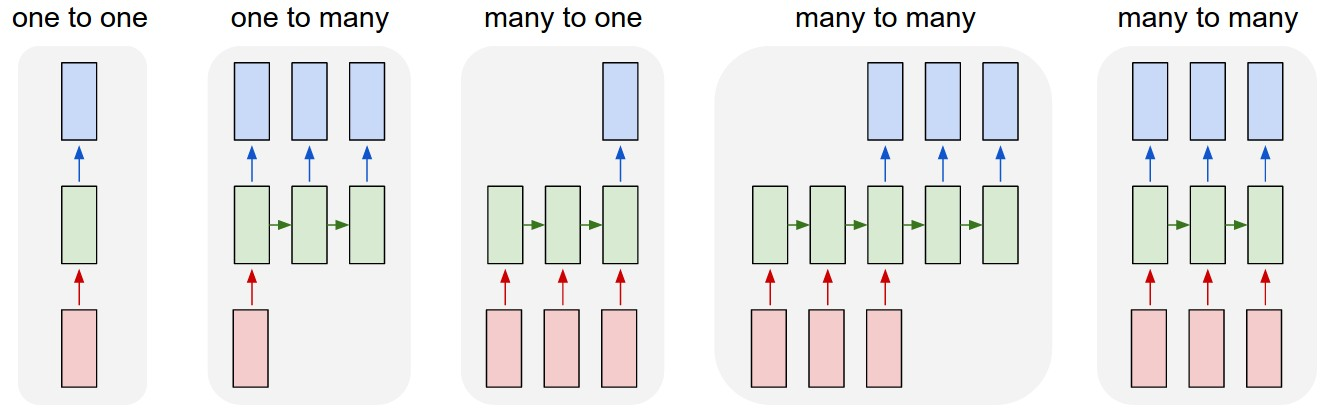
\includegraphics[width=.75\textwidth]{gfx/sequence-prediction-flavors.jpeg}
    \caption{Flavors of sequence prediction~\cite{web:lstm-effectiveness}}
    \label{fig:sequence-prediction-flavors}
\end{figure}

Sequence prediction is a common task in NLP, for example in machine translation or writing novels. The order of input samples is captured, and the prediction is partially based upon it. There are several flavors of it, mostly depending on the number of inputs and outputs, as illustrated in \autoref{fig:sequence-prediction-flavors}. Here, we focus on many-to-many and many-to-one predictions.

A function $predict$ takes in a sequence $seq_{in}$ and gives out an output $\hat{s}$, which can be an itemset or a sequence, depending on the flavor of sequence prediction. The circumflex marks the output as a prediction~\cite{kuhn2013applied}. The following example shows a many-to-many prediction and a many-to-one prediction.

\begin{equation}
\begin{split}
    predict(seq_{in}) &= \widehat{seq_{out}}\\
    predict(seq_{in}) &= \hat{s_k}
\end{split}
\label{eq:prediction-from-sequence}
\end{equation}

Many-to-many predictions are common in the domains of machine translation. For example, the translation of the sentence \textit{"I am writing my master's thesis"} into the german sentence \textit{"Ich schreibe meine Masterarbeit"} can easily be mapped onto the notation previously described. With the alphabet as $\mathscr{I}$ and each itemset representing a single word, the input and target sequences can be noted as:

\begin{equation*}
\begin{split}
seq_{in} &= \langle(I) (am) (writing) (my) (thesis)\rangle\\
\widehat{seq_{out}} &= \langle(Ich) (schreibe) (meine) (Masterarbeit)\rangle
\end{split}
\end{equation*}

Many-to-one predictions are used to generate text and even write simple novels~\cite{web:text-generation-machinelearningmastery, web:text-generation-freecodecamp}. As the name suggests, they predict the next itemset in a sequence:

\begin{equation*}
\begin{split}
seq_{in}  &= \langle(I) (am) (writing) (my)\rangle\\
\hat{s} &= \langle thesis\rangle
\end{split}
\end{equation*}

In this thesis, we focus on many-to-one predictions, because we aim to predict the next activity in a running case based on its trace. To formally bring a sequence understanding onto the process prediction problem, we connect both definitions in \autoref{sec:contrib:case-sequence-understanding}. How neural networks are especially suited for sequence prediction will be explained in the next chapter.

\section{Artificial Neural Networks}\label{sec:artificial-neural-networks}
An artificial neural network (ANN) mimics the inner workings of a human brain in that it is made up of connected nodes referred to as neurons. These neurons are interconnected and act on the incoming signals from each connection. This section first gives background on the general structure of a basic neural network in \autoref{sec:feedforward-networks} and then highlights two enhancements for sequence learning in \autoref{sec:recurrent-networks} and \autoref{sec:lstm}.

\subsection{Feedforward neural networks}\label{sec:feedforward-networks}
The first and most trivial type of ANN is the feedforward neural network~\cite{schmidhuber2015deep}. It is not optimally suited for sequence prediction, but serves as a sufficiently complex example to explain the inner workings of an ANN, and for pointing out why long-short term memory networks are more suited to the task at hand.

\begin{figure}[!htb]
    \centering
    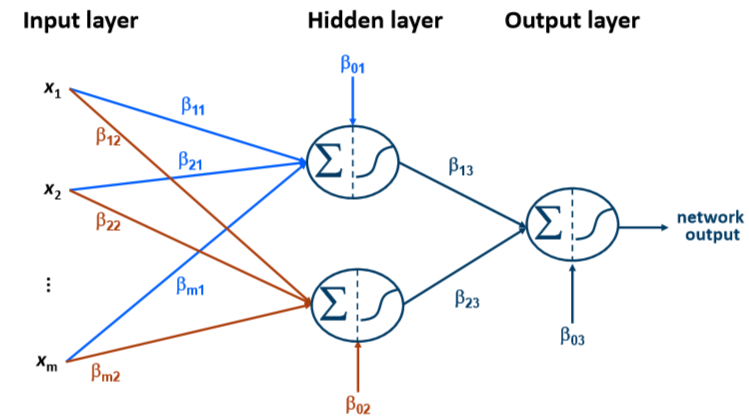
\includegraphics[width=.85\textwidth]{gfx/feedforward-neural-network.png}
    \caption{A feedforward ANN with a single hidden layer~\cite{lessmannBADS}}
    \label{fig:feedforward-ann}
\end{figure}

The nodes in any ANN are organized in layers, with each neuron connecting to every neuron in the adjacent layers, resulting in fully connected layers. The samples are fed into the input layer in the form of a vector of features. The prediction ultimately comes out of the output layer. The layers between the input and output layers are referred to as \textit{hidden layers} and  can be greater in number.

\autoref{fig:feedforward-ann} shows an examplary ANN with a single hidden layer. The features $x_1$ to $x_m$ are fed into the network as one vector, and their numeric values are passed along the edges to every neuron in the next layer. For each neuron, the incoming values are multiplied with the respective edge weight $\beta$ and summed up, as depicted by the $\sum$ symbol in each circle. The sum is passed to a function called \textit{activation function} - illustrated by the sigmoid curve - which controls whether the neuron emits a signal or not. The outputs are passed along the output edges of the respective neurons and the process is repeated for the next layer until the results have reached the output layer. This process of continually feeding the outputs forward to the next layer also gives this type of ANN its name.

The weights $\beta$ are adjusted during training to increase prediction accuracy. For this purpose, the training samples are grouped into \textit{batches}. Once all batches have passed through the network once, an \textit{epoch} has elapsed. The samples in a batch are passed into the network, and the predictions for this batch are compared to the target labels. At this point, the \textit{loss function} calculates how far the network's predictions missed the labels. The weights are then adjusted to reduce the loss in the next batch. Because the goal of the training algorithm is to minimize the network's loss, it can happen that the weights are adapted too well to the training set, making the network overfit.

Overfitting an ANN during training can be avoided by calculating the network's loss both on the training set as well as on the test set. The weight adjustments are made based on the loss on the training set, but the training is stopped once the loss on the test set has ceased to improve for a certain number of epochs. This technique is referred to as early stopping.\\

Because feed-forward ANNs are passing the layer outputs toward the output layer, and the neurons have no memory, this type of network does not to have any capacity for persisting what it has previously processed. However, this is a desirable capability for sequence predictions, as several samples can belong to a single sequence.

The next subsection will show how recurrent neural networks (RNN) have been created with this capacity in mind, making them suited for working with sequential data. Long short-term memory builds on RNNs, and enhances the capacity to remember even further.

\FloatBarrier
\subsection{Recurrent neural networks}\label{sec:recurrent-networks}
As the name suggests, recurrent neural networks (RNN) implement a feedback loop. This loop makes information from the output of a neuron available to itself for the next step. Introducing a time dimension, RNNs are often displayed in an unrolled fashion as in \autoref{fig:rnn-unrolled}. This form of illustration also reveals that recurrent neural networks are intimately related to sequences and lists.

\begin{figure}[!htb]
    \centering
    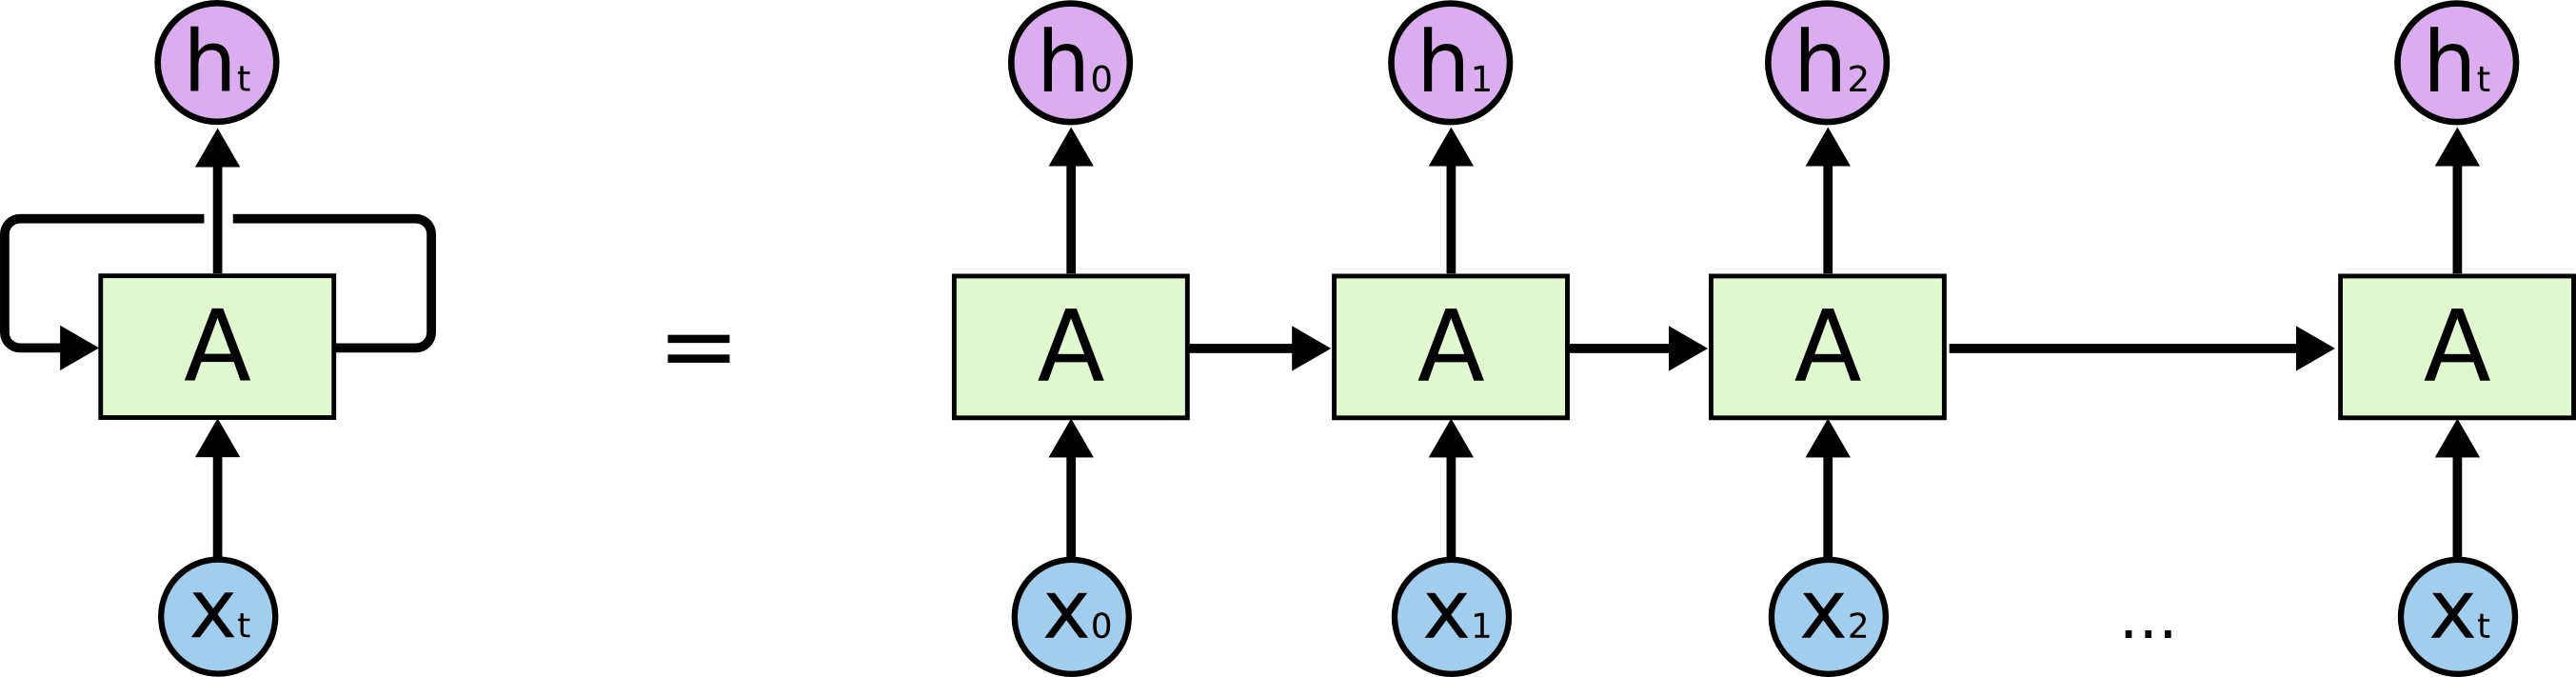
\includegraphics[width=.9\textwidth]{gfx/rnn-unrolled.png}
    \caption{An unrolled neuron of an ANN}
    \label{fig:rnn-unrolled}
\end{figure}

A neuron receives an input $x_t$ and outputs a value $h_t$. The letter $t$ indicates the time dimension. By showing the neuron in an unrolled fashion, it becomes visible that the output of the neuron at time $t$ becomes available to the neuron at time $t+1$~\cite{web:colah}.

The introduction of the time dimension causes the perception of input data to change: It is now required to be three-dimensional. With feedforward ANNs, training data was two-dimensional and consisted of a list of unrelated samples. Samples were the same as a feature vector, but for RNNs, a samples need to be understood as lists of feature vectors. This makes a sample suitable to represent a sequence, because its feature vectors can represent the individual timesteps.

While the loop in an RNN indeed allows recognizing short-term dependencies, the network as a whole will still underperform with long-term dependencies when the gaps between related inputs become too great. The root cause is that RNNs only loop back inputs, and lack a memory to bridge those gaps. This problem has been thoroughly explored by Hochreiter et al.~\cite{hochreiter1991untersuchungen} who also proposed the long short-term memory fix presented in the following subsection.

\subsection{Long short-term memory}\label{sec:lstm}
In recent years, RNNs were applied with great success to a variety of problems: speech recognition, language modeling or translation. This success can be attributed in part to the enhancement of RNNs with long short-term memory (LSTM) cells~\cite{jozefowicz2015empirical,kuhn2013applied,schmidhuber2015deep}.

Hochreiter \& Schmidhuber published this enhancement in 1997~\cite{hochreiter1997} which now sees wide application. Essentially, the repeating neurons of an RNN are turned into cells by equipping them with a cell state $C$, that provides them with the capacity to remember.

\begin{figure}[!htb]
    \centering
    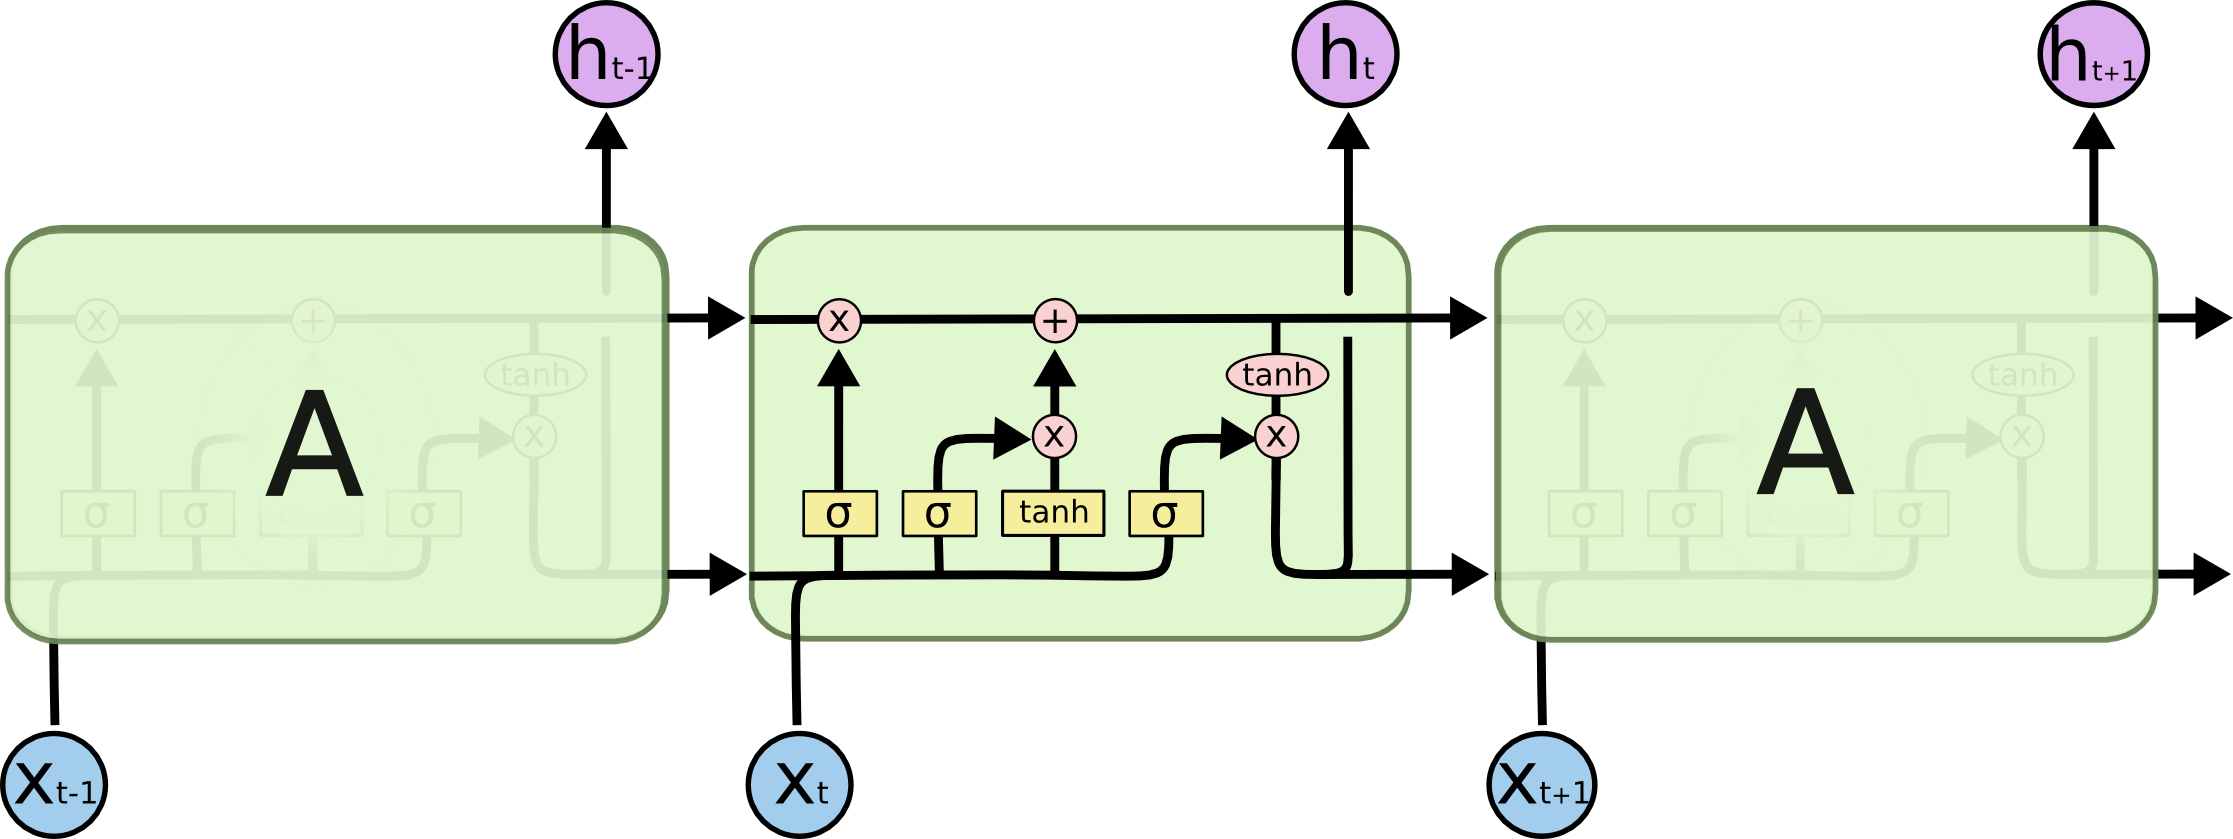
\includegraphics[width=\textwidth]{gfx/lstm-chain.png}
    \caption{An unrolled LSTM cell and its architecture~\cite{web:colah}}
    \label{fig:lstm}
\end{figure}

\autoref{fig:lstm} showcases the architecure of an unrolled LSTM cell. In the diagram, each line carries an entire vector, from the output of one node to the inputs of others. The pink circles represent pointwise operations, like vector addition, while the yellow boxes implement operations. Lines merging denote concatenation, while a line forking denote its content being copied and the copies going to different locations. The cell state $C$ is symbolized by the horizontal upper line running from left to right. The lower line on the left represents $h_{t-1}$, the output of the cell in the previous step.

The $\sigma$ boxes represent gates. Which parts of $C_{t-1}$ to keep and what to forget is decided at the first gate from the left, by taking $h_{t-1}$ and $x_t$ into account. The following $\sigma$ gate and $tanh$ operator together create the update to $C_{t-1}$. Finally on the right, the updated cell state $C_t$ is used together with the activation function $tanh$ to produce the output $h_t$. Variants of this original LSTM cell architecture exist, with most modifications made around the construction of the state $C$ - all exhibiting similar performance~\cite{greff2017lstm}.

\section{Data preparation and feature engineering}
\label{sec:background:feature-engineering}
Data preparation and feature engineering are the tasks in predictive model development that demand the most effort and have the greatest impact on prediction accuracy~\cite{kuhn2013applied}. To assist predictive models during training, most features need to be reformatted. This requirement comes with an implication that can also harm model peformance, which is explained in \autoref{sec:background:curse-of-dimensionality}.
Then, relevant methods used for categorical variables are presentedin \autoref{sec:categorical-feature-engineering}. \autoref{sec:sequential-feature-engineering} points out methods with which to make sequential inputs of various length conform with the fixed-width input requirement of predictive models. In the case of ANNs this requirement can easily be explained by the fixed number of units on the input layer. The methods are demonstrated at the example of the following two sequences:
\begin{equation*}
    \begin{split}
        seq1 &= \langle(Arthur) (is) (the) (king)\rangle\\
        seq2 &= \langle(Maria) (wants) (to) (be) (the) (queen)\rangle
    \end{split}
\end{equation*}

\subsection{The curse of dimensionality}\label{sec:background:curse-of-dimensionality}
\begin{figure}
    \centering
    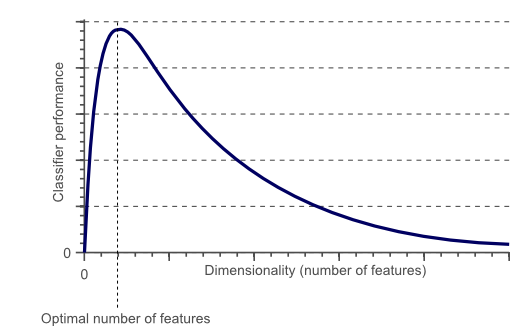
\includegraphics[width=.75\textwidth]{gfx/dimensionality_vs_performance.png}
    \caption[A visualization of the curse of dimensionality]{Adding features to the feature space does not improve model performance indefinitely}
    \label{fig:dimensionality-vs-performance}
\end{figure}
The curse of dimensionality describes a phenomenon that arises when using more and more features~\cite{Aalst2016} with the same number of samples impacts accuracy negatively. It appears across various domains such as combinatorics, sampling optimization and machine learning, and is especially prominent when features are engineered.

The increase in dimensionality caused by the number of features increases the size of the solution space. This eventually causes problems for machine learning algorithms which require statistic significance, and as a result the algorithm becomes less accurate. To counter this effect, more training data would be necessary. Thus, increasing the number of features for training a predictive model only improves accuracy to a certain extent when the number of samples is constant. This relationship is illustrated in \autoref{fig:dimensionality-vs-performance}.

\subsection{Feature engineering for categorical features}\label{sec:categorical-feature-engineering}
While ordinal features are most often normalized, categorical features can be encoded in a variety of ways. Categorical features could be strings like \textit{red} and \textit{black}, which have no numerical format and may or may not be relative to each other. Where one-hot and dictionary encodings are traditional approaches for these features, word embeddings represent a relatively new and promising approach.

\subsubsection*{One-hot encoding}
One-hot encoding is often used for features which have a small to medium-sized number of unique values. Using it, each line item of a feature is expanded to an $n$ column representation, where $n$ represents the number all possible values, also referred to as the alphabet. The columns hold boolean flags, of which only one is ever true in any given row. This type of encoding is also sometimes referred to as "dummy encoding"~\cite{web:pandas-get-dummies}. Thus, the first word of $seq1$ would be encoded as in \autoref{tab:one-hot}. As the alphabet becomes larger, $n$ increases, and the feature vector becomes more sparse. Sparse is a word used to describe data which mostly contains zeros. This characteristic in combination with increasing dimensionality can easily cause symptoms of the curse of dimensionality to appear, which is why it is not used for very large $n$.

\begin{table}[ht]
    \centering
    \begin{tabular}{c|c|c|c|c|c|c|c|c}
        Maria & Arthur & is & wants & to & king & be & the & queen\\
        \hline
        0 & 1 & 0 & 0 & 0 & 0 & 0 & 0 & 0\\
    \end{tabular}
    \caption{One-hot encoding of "Arthur" from alphabet of $seq1$ and $seq2$}
    \label{tab:one-hot}
\end{table}

\subsubsection*{Dictionary encoding}
Widely used in compression, for example in in-memory database systems~\cite{plattner2012memory}, dictionary encoding is also used to encode categorical values. Since predictive models only process numerical values, dictionary encoding is used to create a look-up table and map every value of a feature to a numeric code, like in \autoref{tab:dictionary-encoding}.

In contrast to one-hot encoding, this dictionary encoding does not result in wide and sparse inputs, making it suitable for features with a large number of distinct features. However, it has one important ramification: It imposes an order on features which previously might not have had one. In our example, the condition $Maria > Arthur$ holds true after encoding. The dictionary-encoded sequences would look like this:
\begin{equation*}
    \begin{split}
        seq1 &= \langle1\ 2\ 7\ 5\rangle\\
        seq2 &= \langle0\ 3\ 4\ 6\ 7\ 8\rangle
    \end{split}
\end{equation*}

\begin{figure}
    \centering
    \begin{tabular}{c|ccccccccc}
        Word & Maria & Arthur & is & wants & to & king & be & the & queen\\
        \hline
        Code & 0 & 1 & 2 & 3 & 4 & 5 & 6 & 7 & 8
    \end{tabular}
    \caption{The dictionary built from the $seq1$ and $seq2$}
    \label{tab:dictionary-encoding}
\end{figure}

\subsubsection*{Word embedding}
Because dictionary encodings impose an order and one-hot encodings lead to sparse data, word embeddings are perceived as a viable alternative for encoding categorical variables. Word embeddings are rooted in NLP, where applications deal with very large alphabets.

A word embedding is the output of a neural network with a single hidden layer that has been trained on a large text corpus. It detects how words relate to each other~\cite{web:word-embedding} and puts out highly dimensional vectors for each word. These represent any word property that the model has picked up. In the following example from~\cite{mikolov2013distributed}, the network was able to detect gender properties and social semantics of words:

$$
\vec{v}_{king} - \vec{v}_{man} + \vec{v}_{women} = \vec{v}_{queen}
$$

A word embedding thus allows clustering of words by certain properties. Made popular by Google, word embeddings have motivated numerous publications~\cite{web:ahogrammer, goldberg2014word2vec}. Word embeddings are often available pre-trained on very large text databases, Wikipedia for instance. To use such a pre-trained embedding, the weights from it can be loaded into the respective layer before training the network.

\subsection{Feature engineering for sequences}\label{sec:sequential-feature-engineering}
Predictive model inputs take in feature vectors of fixed size. As shown, sequences can be of arbitrary length, and thus these two requirements collide. To bring variable length inputs into a usable format for predictive models, several methods of formatting have been invented. As some of their names suggest, these come from the domain of Natural Language Processing (NLP), but can easily be transferred to the problem at hand.

\subsubsection*{Sliding Window}
The sliding window format is very common in the areas of NLP and Time Series Forecasting. The sequences are divided into chunks of width $c$. This results in several input tuples for every sequence, and creates the desired tabular format for feeding into the model - illustrated in \autoref{tab:sliding-window}.

\begin{table}
    \centering
    \begin{tabular}{cc}
        Word 1 & Word 2\\
        \hline
        Arthur & is\\
        is & the\\
        the & king\\
        Maria & wants\\
        wants & to\\
        to & be\\
        be & the\\
        the & queen
    \end{tabular}
    \caption{Windows created from $seq1$ and $seq2$ with $c=2$}
    \label{tab:sliding-window}
\end{table}

\subsubsection*{Bag-Of-Words}
The bag-of-words (BOW) encoding produces $l$ input tuples, where $l$ is the length of the encoded sequence. Similarly to one-hot encoding, the alphabet needs to be known. One arrives at the encoding by marking the occurrence of each item in the alphabet for each subsequence $seq_{1,k}$. $k$ is incremented for every sample from 1 to $l$, making the feature vector fill up with truth values as $k$ gets larger. As \autoref{tab:bow-encoding} evidences, this type of encoding results in sparse data, too.

\begin{table}
    \centering
    \begin{tabular}{c|ccccccccc}
        Sequence & Maria & Arthur & is & wants & to & king & be & the & queen\\
        \hline
        $seq1_{1,1}$ & 0 & 1 & 0 & 0 & 0 & 0 & 0 & 0 & 0\\
        $seq1_{1,2}$ & 0 & 1 & 1 & 0 & 0 & 0 & 0 & 0 & 0\\
        $seq1_{1,3}$ & 0 & 1 & 1 & 0 & 0 & 0 & 0 & 1 & 0\\
        $seq1_{1,4}$ & 0 & 1 & 1 & 0 & 0 & 1 & 0 & 1 & 0\\
        \hline
        $seq2_{1,1}$ & 1 & 0 & 0 & 0 & 0 & 0 & 0 & 0 & 0\\
        $seq2_{1,2}$ & 1 & 0 & 0 & 1 & 0 & 0 & 0 & 0 & 0\\
        $seq2_{1,3}$ & 1 & 0 & 0 & 1 & 1 & 0 & 0 & 0 & 0\\
        $seq2_{1,4}$ & 1 & 0 & 0 & 1 & 1 & 0 & 1 & 0 & 0\\
        $seq2_{1,5}$ & 1 & 0 & 0 & 1 & 1 & 0 & 1 & 1 & 0\\
        $seq2_{1,5}$ & 1 & 0 & 0 & 1 & 1 & 0 & 1 & 1 & 1\\
    \end{tabular}
    \caption{Bag-of-words encoding for $seq1$ and $seq2$}
    \label{tab:bow-encoding}
\end{table}
\subsubsection*{$n$-grams}
The $n$-gram approach is very popular in computational linguistics, biology and data compression and is effectively an $(n-1)$-order Markov model, with the most popular choices for $n$ being $1,2$ and $3$. These models would be called \textit{unigram}, \textit{bigram} and \textit{trigram} models.

Similar to BOW, an $n$-gram model counts occurences. Different from BOW however, it tracks the occurence of subsequences of length $n$. Suppose a set $LS$ holds all possible values of a single feature. From $LS$, a feature set $FS$ is constructed with every item being a permutation of length $n$. A feature in this set would be referred to as \textit{gram}, and can also be understood as a possible subsequence.

$$
FS = S(LS, n)
$$

While $n$-grams can be be powerful features to use, their high dimensionality causes high computational loads and sparse data. With the small feature set of 9 words in the given example, a line item using tri-grams would already be $\frac{|FS|!}{(|FS|-n)!}=504$ elements wide.

\subsubsection*{subsequence mining}
One of the main weaknesses of $n$-grams is the restriction to a single $n$ and that "one may need to examine a combinatorially explosive
number of possible subsequence patterns" \cite{pei2001prefixspan}. For this reason, approaches have been developed that combine the benefit of $n$-grams with more flexibility by avoiding the limitation to $n$. An algorithms sifts through input sequences and detects sequential patterns of any length. These sequences are then encoded instead of the $n$-grams, resulting in line items similar to the ones in \autoref{tab:bow-encoding}, with the respective boolean entry denoting the occurence of a specific subsequence in the sequence. Examples for these algorithms are GSP \cite{srikant1996gsp}, FreeSpan \cite{han2000freespan} and PrefixSpan \cite{pei2001prefixspan}.\\

For every mined subsequence $ss$, the \textit{support} metric $supp(ss)$ can be calculated. This metric indicates in how many complete sequences, $ss$ as a subsequence. Sometimes, shorter subsequences are part of longer subsequences, like $ss1$ is contained in $ss2$:

\begin{equation*}
\begin{split}
s1 &= (a,d)\\
s2 &= (a,d,c)
\end{split}
\end{equation*}

If the condition $supp(ss1) > supp(ss2)$ holds true, then $ss1$ is called a \textit{closed} subsequence as it can not be expanded without shrinking its support.
